% @Author: Jacem Chaieb
% @Date:   2015-07-26 13:42:06
% @Last Modified by:   Jacem Chaieb
% @Last Modified time: 2016-04-12 15:45:38

%%%%%%%%%%%%%%%%%%%%%%%%%%%%
% CHAPTER                  %
%%%%%%%%%%%%%%%%%%%%%%%%%%%%

\chapter{General framework of the project}%


%%%%%%%%%%%%%%%%%%%%%%%%%%%%
% SECTION                  %
%%%%%%%%%%%%%%%%%%%%%%%%%%%%
\section*{Introduction}
We begin this chapter with a general presentation of the organization
of the reception. We will then detail the context and the problem of our project and
the proposed solution, which will attempt to resolve the inconveniences
that already exist. We will finish this chapter by describing
the schedule of our internship through the Gantt chart as well as the
development process.\\

\section{Presentation of the host organization}
TechLead is a Tunisian IT engineering company whose mission is to design and implement Salesforce solutions for companies to improve their productivity, profitability, and market adaptability.\\
The company supports its clients throughout the life cycle of their projects, from consulting to the complete implementation of the solution and up to the transfer of skills. The company's young, dynamic, and versatile team assists clients in all stages of implementing their Salesforce solution to better interact with customers, partners, and prospects.
The company offers many services such as:
\begin{itemize}
\item[•] \textbf{Accompaniment:} The company's Salesforce advisors help clients implement and develop your Salesforce solution. They can intervene in the audit and analysis of needs, the design, the integration of data, and the configuration of clients' projects quickly and efficiently.
\item[•] \textbf{Support:} The company's experienced developers can provide assistance and maintenance to clients' projects in the various administration or development needs with good availability and responsiveness.
\item[•] \textbf{Salesforce Training:} The company provides training tailored to clients' needs and helps them use and leverage the capabilities of Salesforce.
\end{itemize}
\begin{figure}[H]%
    \center   
    
\includegraphics[scale=0.2]{techlead.png}
    \caption*{Host organization TECHLEAD}
\end{figure}



\section{Project presentation}
In this part, we put our work in its general context.
first, we present the context. Second, we present the problem and the reasons for suggesting this topic. Third, we present the solution
proposed to solve the problem. Finally, we will describe the objectives
of this project.
\subsection{Context}
Salesforce is a highly customizable advanced CRM, it stores customer data, gives processes to nurture prospective customers, and provides ways to collaborate with other workers. \cite{1} \\
Salesforce comes with a lot of standard functionality, or out-of-the-box products and features that clients can use to run their business. Here are some common things businesses want to do with Salesforce and the features Salesforce gives that support those activities:\cite {1}
\begin{figure}[H]%
    \center   
    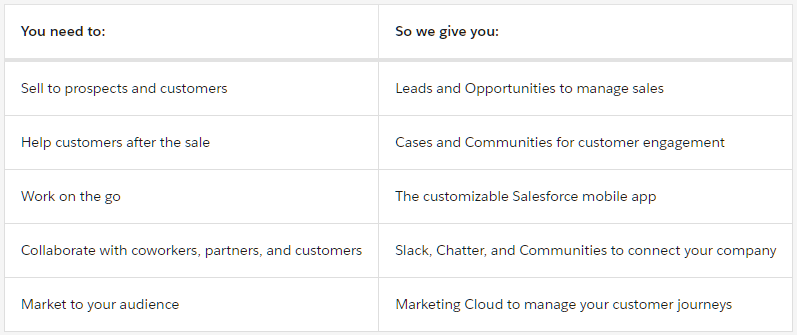
\includegraphics[scale=0.8]{context.png}
    \caption{Salesforce features, Source: \cite{1}}
\end{figure}
The platform also helps clients move fast. Part of that speed comes from replacing tasks that clients are used to doing by hand with more streamlined processes.\cite{2}\\
The platform's goal is to make big changes with minimal effort and to solve mistakes that impact the buyer using dynamic expandable interfaces using additional extensions.
\begin{figure}[H]%
    \center   
    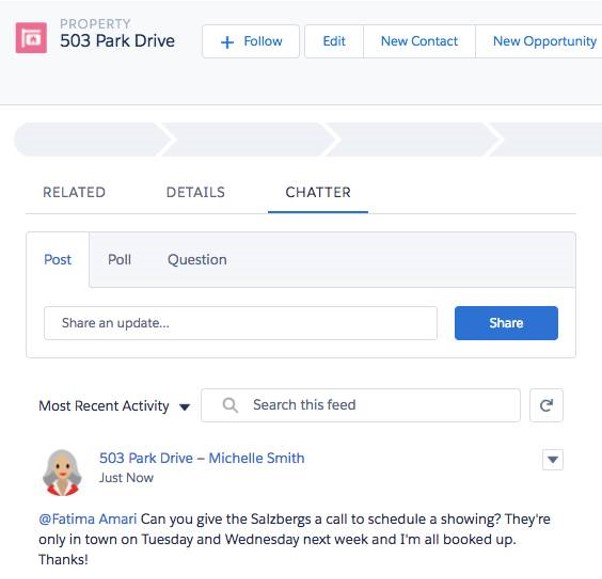
\includegraphics[scale=0.8]{chatter.jpg}
    \caption{Chatter extension in Salesforce, Source: \cite{2}}
\end{figure}
\newpage
Here are a few use cases for different departments:
\begin{figure}[H]%
    \center   
    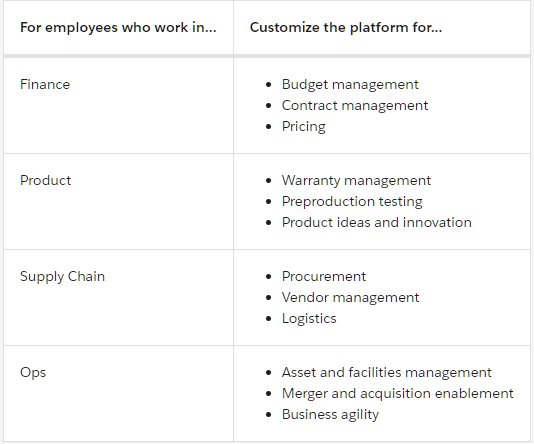
\includegraphics[scale=0.8]{usecases.png}
    \caption{Usecases for Salesforce, Source: \cite{2}}
\end{figure}
Salesforce is a cloud company. Everything to offer resides in the trusted, multitenant cloud.\\
The Salesforce platform is the foundation of the services. It’s powered by metadata and made up of different parts, like data services, artificial intelligence, and robust APIs for development.  \\
All the apps sit on top of the platform. The prebuilt offerings like Sales Cloud and Marketing Cloud, along with apps built using the platform, have consistent, powerful functionality.\\
Everything is integrated. The platform technologies like predictive analytics and the development framework are built into everything to offer and everything to build.\cite{3} 
\begin{figure}[H]%
    \center   
    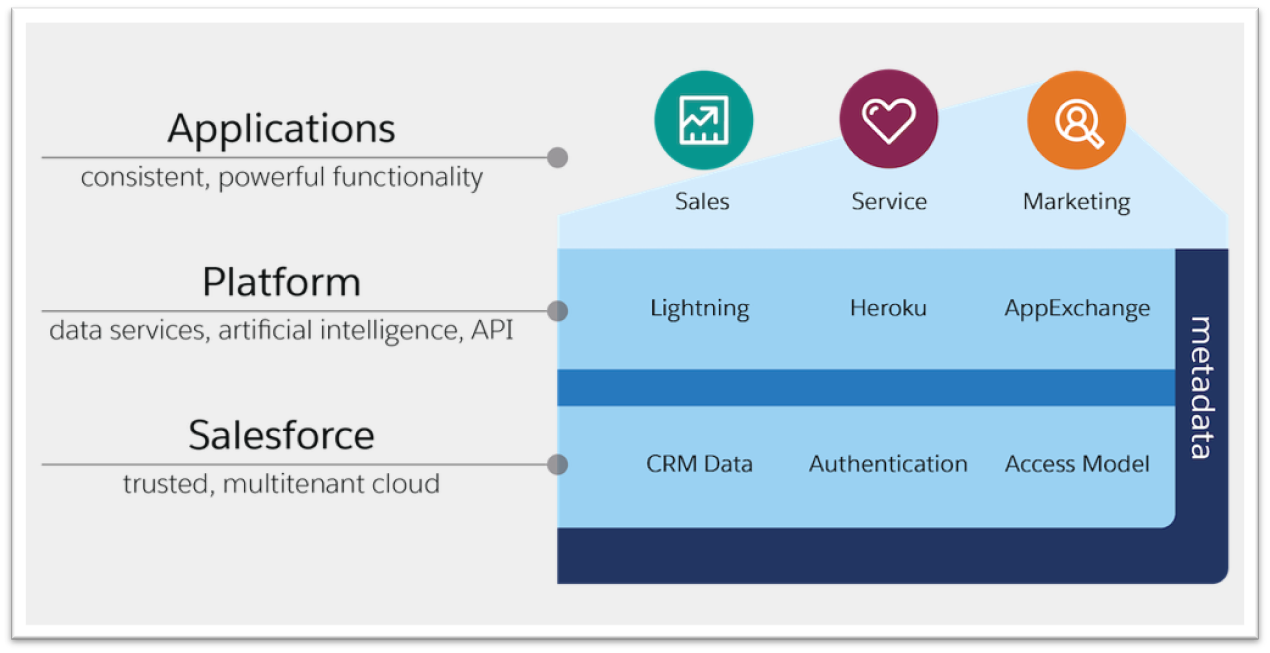
\includegraphics[scale=0.8]{architecture.png}
    \caption{Salesforce's architecture, Source: \cite{3}}
\end{figure}

\subsection{Problem}
In Salesforce, each user is identified by a unique username and profile. Along with other settings, the profile determines what tasks a user can perform, what data they can view, and how they can use the data.\\
As a Salesforce admin, you manage users in your organization. In addition to creating and assigning users, user management includes managing permissions and licenses, delegating users, and more \\

Users are managed in the community through a Salesforce interface and over several stages, making it difficult and time-consuming.\\
This problem becomes even more apparent when dealing with the base Salesforce interface where there are so many places to go when trying to manage even the simplest tasks regarding users and their communities for example:
\begin{itemize}
\item[•] If the administrator wants to manage all his users he will have to access the Salesforce setup home menu but when accessing his community users he will have to access the community administration interface that takes so much time to load.
\item[•] If the administrator wants to track members’ connection history, it cannot be done without using third-party extensions or applications.
\item[•] If the administrator wants to add multiple members at once to his community, it cannot be done without wasting time navigating between interfaces.
\end{itemize}
 

\subsection{Proposed solution}
The main objective of our work is to design and develop a powerful tool to facilitate the task of managing the users of the community.\\
This application is intended to offer any organization a simple and effective means to manage the "administration" part, then the connection history part, and finally provide a synthetic dashboard visualizing the KPIs as well as a smart Chatbot solution for the administrators and community managers.
\subsection{Objectives}
Ensure user satisfaction by ensuring:\\
\textbf{Functional objectives:}
\begin{enumerate}
\item \textbf{Choice of the community:}
Select the community to which we will manage the users

\item \textbf{Manage users:}
The system must allow users to be managed with the functionalities of activation,
deactivation, modification, and consultation of the list of users via a data table.
Creation of different filters that allow us to facilitate the navigation of the list of users.

\item \textbf{Manage connection history:}
Create a chart that shows the number of user connections per day, week, year, or
according to a well-determined date. This allows the administrator to modify the user’s license

\item \textbf{Offer a synthetic dashboard}
\item \textbf{Offer a smart Chatbot solution}

\end{enumerate}
\textbf{Non-functional objectives:}
\begin{enumerate}
\item\textbf{ Security:} Access to information is only possible after verification of privileges and access rights,
for example Authentication, Redirections.

\item \textbf{Ergonomics and user-friendliness:}
The application will provide a user-friendly and easy-to-use interface that does not
require any prerequisites, so it can be used by all types of users (even non-computer specialists).

\item \textbf{Extensibility and maintainability:}
The architecture of the application will allow the evolution and maintenance (addition
or deletion or update) at the level of its various modules in a flexible manner.

\item \textbf{Performance:}
The application must be efficient, i.e. the system must react within a period that does
not exceed 5 seconds, whatever the action of the application.
\item \textbf{Availability:}
The application will be available on 24/24 and 7/7 except during maintenance.

\end{enumerate}
\textbf{Technical objectives:}
\begin{enumerate}
\item Organization of the application according to the MVC(Model-View-Controller) architecture: a software architecture model that separates the representation of information from the user's interaction with it.

\begin{figure}[H]%
    \center   
    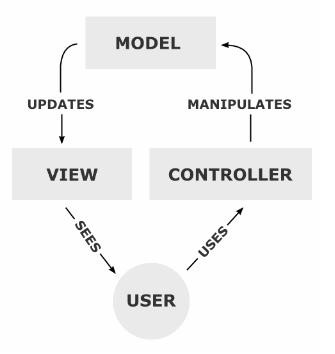
\includegraphics[scale=0.8]{mvc.jpg}
    \caption{MVC Architecture, Source: \cite{6}}
\end{figure}

\item Using the Framework "LWC".
\item Using the programming language "Apex".
\item Using the library "SLDS".
\item Using the Salesforce Object Query Language "SOQL/SOSL".

\end{enumerate}
\section{Study of the existing}

In this part, we analyze and criticize the existing applications
currently, through the table \ref{existing_table}, we propose a solution that solves
their drawbacks.\\
While searching for existing solutions for our main problem we came across 3 of the most popular applications and Salesforce extensions specializing in users and community management:
\begin{itemize}
\item[•] \textbf{HubSpot:} HubSpot is a popular marketing, sales, and customer service platform that integrates with Salesforce. 
\begin{figure}[H]%
    \center   
    
\includegraphics[scale=0.5]{hubspot.png}
    \caption*{HubSpot Logo}
\end{figure}
HubSpot uses Salesforce's user management features to allow organizations to manage their teams and control access to different parts of the application.
\begin{figure}[H]%
    \center   
    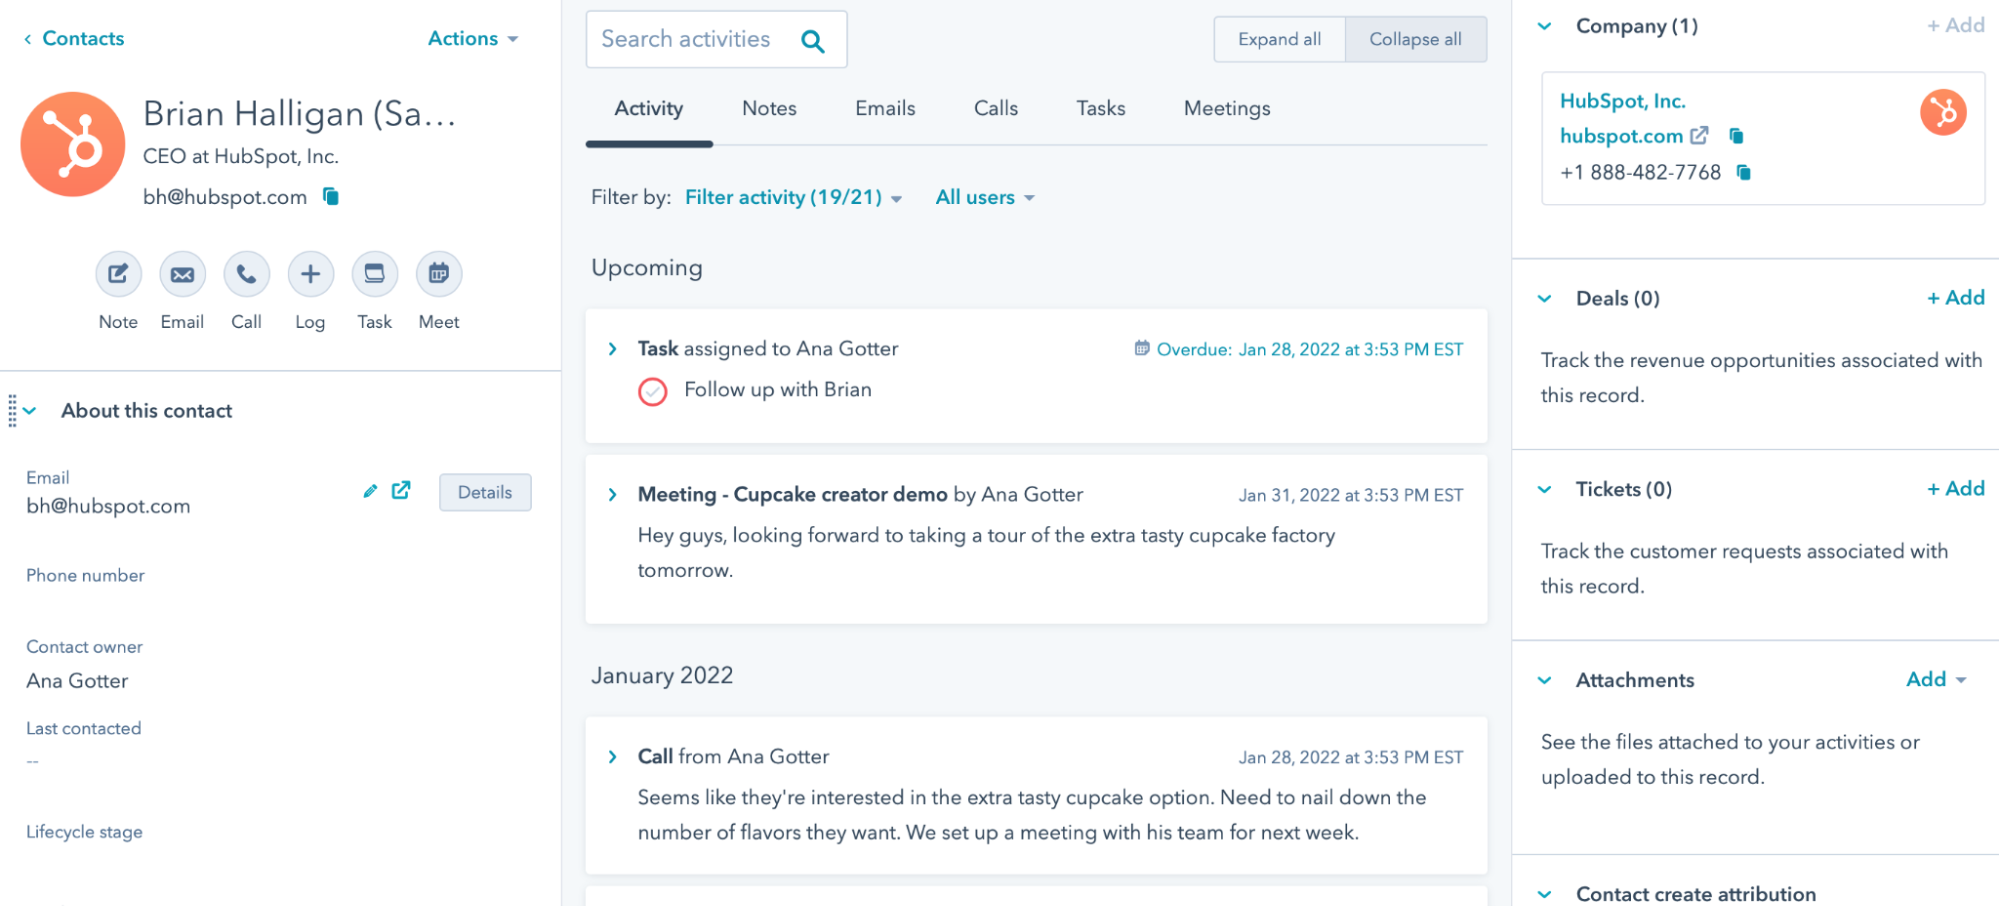
\includegraphics[scale=0.2]{hubspot_ui.png}
    \caption{HubSpot user interface}
\end{figure}
\item[•] \textbf{ZenDesk:} ZenDesk is a customer support platform that integrates with Salesforce. 
\begin{figure}[H]%
    \center   
    
\includegraphics[scale=0.5]{zendesk.png}
    \caption*{ZenDesk Logo}
\end{figure}
ZenDesk uses Salesforce's user management features to allow organizations to manage their support teams and control access to different parts of the application.
\begin{figure}[H]%
    \center   
    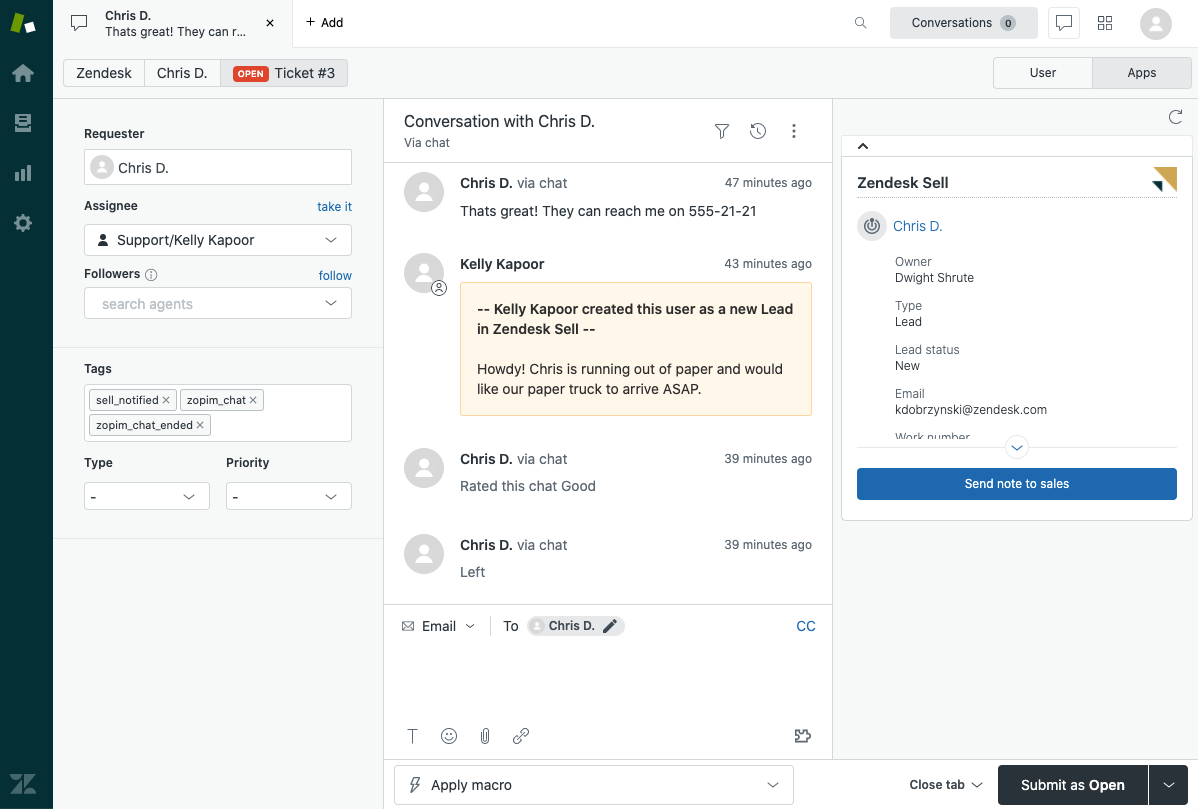
\includegraphics[scale=0.3]{zendesk_ui.png}
    \caption{ZenDesk user interface}
\end{figure}
\pagebreak
\item[•] \textbf{Conga:} Conga is a document generation and reporting platform that integrates with Salesforce. 
\begin{figure}[H]%
    \center   
    
\includegraphics[scale=0.5]{conga.png}
    \caption*{Conga Logo}
\end{figure}
Conga uses Salesforce's user management features to allow organizations to manage their teams and control access to different parts of the application.
\begin{figure}[H]%
    \center   
    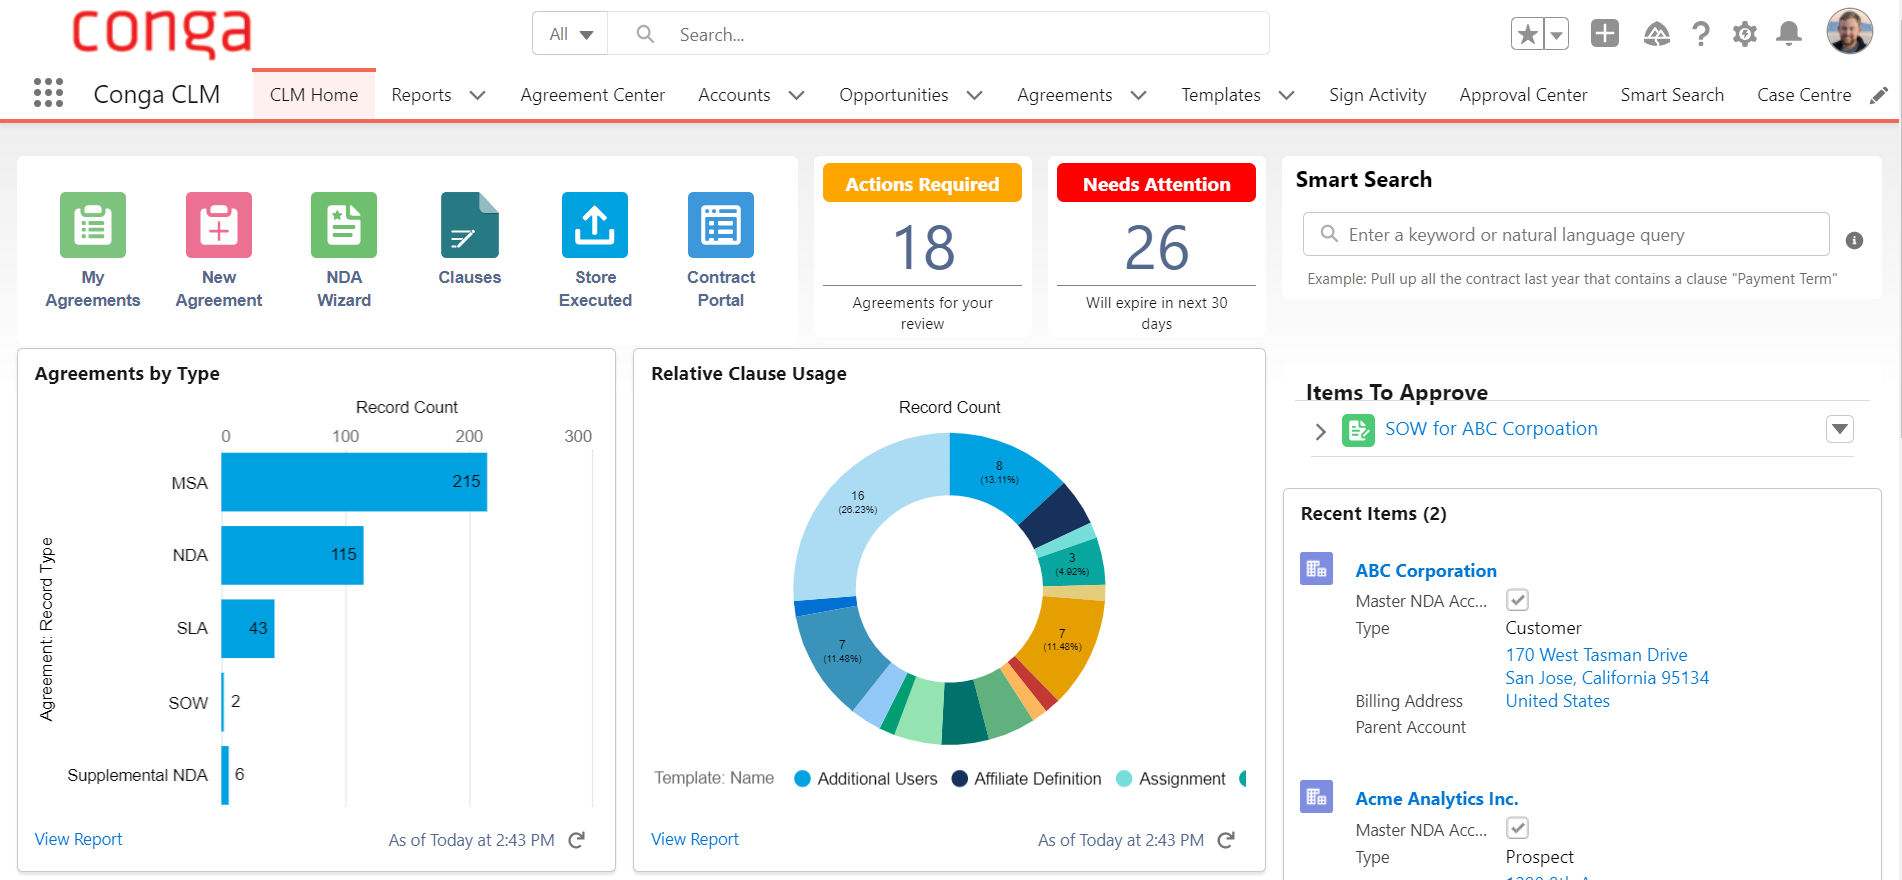
\includegraphics[scale=0.3]{conga_ui.png}
    \caption{Conga user interface}
\end{figure}
\end{itemize}
\begin{table}[H]
\begin{tabular}{|l|l|l|}
\hline
\textbf{Application} & \textbf{Pros}                                                                                                                                                                                                                                                                                                       & \textbf{Cons}                                                                                                                                                                                                                                                                                                                                                                                           \\ \hline
HubSpot              & \begin{tabular}[c]{@{}l@{}}- User-Friendly Interface\\ - Ability to create custom roles\\ and assign specific permissions\\ to users based on their roles.\\ - Ability tracks user activity,\\ allowing businesses \\ to monitor user behavior.\end{tabular}                                                        & \begin{tabular}[c]{@{}l@{}}- Interface can be complex, \\ particularly for businesses \\ with a large number of users.\\ - Pricing structure is based\\ on the number of contacts\\ in a business's database,\\ which can make it more expensive\\ for businesses with larger teams.\\ - There may be a learning curve\\ when it comes to managing users\\ and configuring access control.\end{tabular} \\ \hline
ZenDesk              & \begin{tabular}[c]{@{}l@{}}- Provides user analytics,\\ allowing businesses \\ to monitor user behavior.\\ - Allows businesses to set up\\ custom notifications for user actions,\\ such as ticket creation or update.\\ - Provides tools for user collaboration,\\ such as shared views and comments.\end{tabular} & \begin{tabular}[c]{@{}l@{}}- May not offer as much granularity\\ as some businesses require.\\ - Interface may not offer \\ as much customization \\ as some businesses require.\\ - Pricing structure is based\\ on the number of agents,\\ which can make it more expensive\\ for businesses with larger teams.\end{tabular}                                                                          \\ \hline
Conga                & \begin{tabular}[c]{@{}l@{}}- Offers customizable workflows.\\ - Offers Centralized \\ user management system.\\ - Provides tools for user collaboration,\\ such as document sharing and commenting\end{tabular}                                                                                                     & \begin{tabular}[c]{@{}l@{}}- Limited third-party integrations\\ - Pricing structure can be\\ more expensive for \\ businesses with larger teams.\\ - User management interface\\ can be complex.\end{tabular}                                                                                                                                                                                           \\ \hline
\end{tabular}
\caption{Study of the existing}
\label{existing_table}
\end{table}
\section{Development process}
A software development process is a set of related activities
followed by a team led to the production of the software within the organization. It consists of a detailed plan describing how to develop, design,
test, deploy, and maintain the product. \cite{4}
\subsection{Incremental development}

In this context, we adopt the process of incremental development as an approach to the realization of our project. According to this process, the customer's needs are specialized, the software is globally designed,
then the realization is done by an increment of functionalities. \\
Each increment
is considered an executable part of the final system. These increments
are successively integrated into the final product and at each stage, the software is
tested, operated, and maintained as a whole. \\
Implementing the software by
increment makes it possible to take into account the risk analysis to facilitate
the detection of errors at the earliest according to customer feedback and to reduce
the time and cost of production, which helps in the realization of software
quality.\\
Incremental development is a preferred approach in Salesforce application development for several reasons:
\begin{enumerate}
\item \textbf{Iterative Process:} Incremental development follows an iterative process where the development is divided into small, manageable phases. Each phase focuses on delivering a specific set of features or functionalities. This approach allows for frequent feedback and collaboration with stakeholders, ensuring that their evolving requirements are met throughout the development process.
\item \textbf{Faster Time-to-Market:} By breaking down the development into smaller increments, we can release functional versions of the application more quickly. This enables organizations to deploy and start using essential features earlier, gaining a competitive advantage and generating value sooner.
\item \textbf{Adaptability to Changing Requirements:} The business landscape is dynamic, and requirements can change rapidly. Incremental development allows for flexibility and adaptability, as it enables us to respond to changing needs and incorporate new features or adjustments easily. It reduces the risk of building a solution that doesn't align with evolving business requirements.
\item \textbf{Risk Mitigation:} Incremental development minimizes risk by addressing potential issues early in the development cycle. With each iteration, we can identify and rectify any problems, ensuring that the final product meets quality standards. It also allows for better risk management and course correction during the development process.
\item \textbf{Scalability and Maintainability:} Incremental development makes it easier to manage the scalability and maintainability of Salesforce applications. By building and releasing smaller increments, it becomes simpler to identify and resolve scalability issues as the application evolves. Additionally, the iterative nature of development allows for ongoing improvements and enhancements, ensuring the application remains maintainable and adaptable in the long term.
\end{enumerate}





\subsection{Provisional schedule of tasks}
A Gantt chart is a graphical tool that represents the management
of the project over time, which facilitates its implementation.\\
Indeed, the internship within TECHLEAD will run for 4 months. The figure \ref{timeline} illustrates a provisional schedule set early in development, representing the main stages leading to a functional solution that meets the criteria defined by previously mentioned specifications.

\begin{figure}[H]%
    \center   
    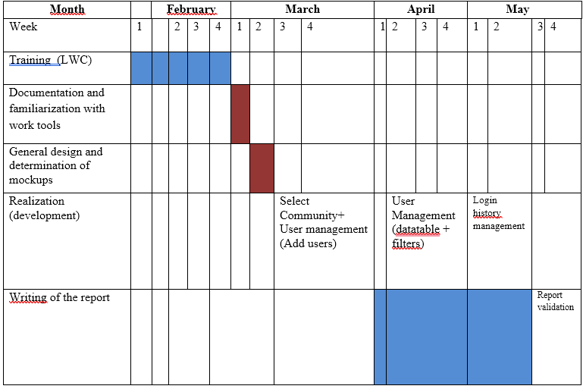
\includegraphics[scale=1]{gantt.png}
    \caption{Gantt diagram}
    \label{timeline}
\end{figure}
\section*{Conclusion}
In this chapter, we have introduced the context of our project by representing the host organization in the first place. Secondly, we have introduced the sales platform and its features. Thirdly, we have
cleared up the problem. Then, we described the proposed solution and
the objectives to be achieved. After that, we analyzed the existing applications. Lastly, we have depicted the advancement of
activities throughout the project according to the adopted development process.
In the next chapter, we will specify the functional requirements and the
non-functional needs.